% Derived from the template file for the LaTeX package SVJour3
% for Springer journals.          Springer Heidelberg 2010/09/16
%
% This template includes a few options for different layouts and
% content for various journals. Please consult a previous issue of
% your journal as needed.
%
% First comes an example EPS file -- just ignore it and
% proceed on the \documentclass line
% your LaTeX will extract the file if required
\begin{filecontents*}{example.eps}
%!PS-Adobe-3.0 EPSF-3.0
%%BoundingBox: 19 19 221 221
%%CreationDate: Mon Sep 29 1997
%%Creator: programmed by hand (JK)
%%EndComments
gsave
newpath
  20 20 moveto
  20 220 lineto
  220 220 lineto
  220 20 lineto
closepath
2 setlinewidth
gsave
  .4 setgray fill
grestore
stroke
grestore
\end{filecontents*}
%
\RequirePackage{fix-cm}
%
%\documentclass{svjour3}                     % onecolumn (standard format)
%\documentclass[smallcondensed]{svjour3}     % onecolumn (ditto)
\documentclass[smallextended]{svjour3}       % onecolumn (second format)
%\documentclass[twocolumn]{svjour3}          % twocolumn
%
\smartqed  % flush right qed marks, e.g. at end of proof
%
\usepackage{graphicx}
%
% \usepackage{mathptmx}      % use Times fonts if available on your TeX system
%
% insert here the call for the packages your document requires
\usepackage{amsmath}
\usepackage{amssymb}
\usepackage{array}
\usepackage{hhline}
\usepackage{mathtools}
\usepackage{multirow}
\usepackage{tikz}
\usetikzlibrary{arrows, calc, decorations.pathreplacing, positioning,
  shapes.geometric}
% etc.

\usepackage{attrib}
\usepackage{csquotes}

\usepackage{graphicx}
\graphicspath{ {support/} }

% please place your own definitions here and don't use \def but
% \newcommand{}{}

% For example theory of lists
\newcommand{\function}{\rightarrow}
\newcommand{\Zero}{\text{Z}}
\newcommand{\Succ}{\text{S}}
\newcommand{\List}{\text{List}}
\newcommand{\ListA}{\text{List} \  a}
\newcommand{\Nil}{\text{Nil}}
\newcommand{\Cons}{\text{Cons}}
\newcommand{\Head}{\text{head}}
\newcommand{\Tail}{\text{tail}}
\newcommand{\Append}{\text{append}}
\newcommand{\Reverse}{\text{reverse}}
\newcommand{\Length}{\text{length}}
\newcommand{\Map}{\text{map}}
\newcommand{\Foldl}{\text{foldl}}
\newcommand{\Foldr}{\text{foldr}}

% For interestingness table
\newcommand{\iE}{\textbf{E}}
\newcommand{\iN}{\textbf{N}}
\newcommand{\iS}{\textbf{S}}
\newcommand{\iA}{\textbf{A}}
\newcommand{\iC}{\textbf{C}}
\newcommand{\iU}{\textbf{U}}
\newcommand{\tIFF}{if-and-only-if}
\newcommand{\tNE}{non-exists}
\newcommand{\tIMP}{implies}
\newcommand{\tRow}[1]{#1 \\ \hline}

% Insert the name of "your journal" with
\journalname{Journal of Automated Reasoning}

\begin{document}

\title{Quantitative Benchmarking for Automatically Generated Conjectures%\thanks
% {Grants or other notes about the article that should go on the front page
% should be placed here. General acknowledgments should be placed at the end of
% the article.}
}
% \subtitle{Do you have a subtitle?\\ If so, write it here}

% \titlerunning{Short form of title}        % if too long for running head

\author{Chris Warburton \and
        Alison Pease
        % TODO: Invite Katya? Even if she only offers some help, can acknowledge
}

% \authorrunning{Short form of author list} % if too long for running head

\institute{C. Warburton \at
           University of Dundee \\
           \email{c.m.warburton@dundee.ac.uk}           %  \\
%             \emph{Present address:} of F. Author  %  if needed
           \and
           A. Pease \at
           University of Dundee \\
           \email{a.pease@dundee.ac.uk}
}

\date{Received: date / Accepted: date}
% The correct dates will be entered by the editor

\maketitle

% Look carefully at each system's (paper's) eval section

% Make it clear that methodology is the point (it's not just a detail, like in a
% chemistry paper for example)

\begin{abstract}
  We propose a benchmark suite for evaluating the efficiency and effectiveness
  of automated tools for \emph{theory exploration} or
  \emph{conjecture formation} in higher-order, inductive theories; a domain
  especially suited for analysing software. By providing standard tools and
  metrics, we hope to encourage innovation and comparison between the disparate
  approaches currently being pursued, and spur improvements similar to those
  seen in the competitive field of automated theorem proving.
%\keywords{First keyword \and Second keyword \and More}
% \PACS{PACS code1 \and PACS code2 \and more}
% \subclass{MSC code1 \and MSC code2 \and more}
\end{abstract}

\section{Introduction}
\label{intro}

% Lay out the field of TE: motivation, systems, evaluation, problems...

\emph{Automated theory exploration} (ATE), also known as
\emph{conjecture generation/formation}, is the open-ended problem of producing
conjectures about a given logical theory which are somehow ``interesting''.

This has applications wherever we find use for formal statements: in proof
assistants and their libraries, in mathematics education and research, and
(of special concern for the authors) in the specification, verification,
optimisation and testing of software.

Existing attempts at tackling this problem are difficult to compare, due
partially to the variety of approaches taken, but also because of the inherent
ambiguity of the task and the different goals emphasised by their designers and
their choice of evaluation method.

We attempt to solve this discrepancy, at least for the foreseeable future, by
defining a standard, unambiguous benchmarking approach with which to compare
ATE systems. Our contributions include:

\begin{itemize}
\item A general methodology for benchmarking ATE systems.
\item Resolving the issue of ``interestingness'' through the use of
  theorem-proving benchmarks as a ground-truth.
\item A specific instantiation of this methodology, using the Tons of Inductive
  Problems benchmark as a corpus.
\item Automated tooling to perform this benchmarking.
\item Application of our methodology to the QuickSpec and IsaCoSy ATE systems,
  and a discussion of the results.
\end{itemize}

Section \ref{sec:background} describes the ATE problem in more detail, along
with existing approaches and their evaluation methodologies. We explain our
proposal for a more general benchmark in section \ref{sec:proposal} and
section \ref{sec:application} shows the results when applied to existing ATE
tools. Analysis of these results is given in section \ref{sec:discussion} and
concluding remarks in \ref{sec:conclusion}.

%- Existing approaches are difficult to compare
% - They want different things
% - They're evaluated differently
% - They're evaluated ``locally'' (as white boxen)

% Look at phd symposium 2017, moa's conjecture synthesis paper, etc.
% We can just jump straight in to automated conjecture generation

\section{Background}
\label{sec:background}

\subsection{Motivation}
\label{sec:motivation}

% more detail about evaluation, interestingness, etc. Reference Simon/Alan
% interestingness, e.g. examples from textbooks, etc.

\begin{figure}
  \begin{equation*}
    \begin{split}
      \forall a. \Nil            &: \ListA                                  \\
      \forall a. \Cons           &: a \rightarrow \ListA \rightarrow \ListA \\
      \Head(\Cons(x, xs))        &= x                                       \\
      \Tail(\Cons(x, xs))        &= xs                                      \\
      \Append(\Nil,         ys)  &= ys                                      \\
      \Append(\Cons(x, xs), ys)  &= \Cons(x, \Append(xs, ys))               \\
      \Reverse(\Nil)             &= \Nil                                    \\
      \Reverse(\Cons(x, xs))     &= \Append(\Reverse(xs), \Cons(x, \Nil))   \\
      \Length(\Nil)              &= \Zero                                   \\
      \Length(\Cons(x, xs))      &= \Succ (\Length(xs))                     \\
      \Map(f, \Nil)              &= \Nil                                    \\
      \Map(f, \Cons(x, xs))      &= \Cons(f(x), \Map(f, xs))                \\
      \Foldl(f, x, \Nil)         &= x                                       \\
      \Foldl(f, x, \Cons(y, ys)) &= \Foldl(f, f(x, y), xs)                  \\
      \Foldr(f, \Nil,         y) &= y                                       \\
      \Foldr(f, \Cons(x, xs), y) &= f(x, \Foldr(f, xs, y))
    \end{split}
  \end{equation*}
  \caption{A simple theory defining a $\List$ type and some associated
    operations. $\Zero$ and $\Succ$ are from a Peano encoding of the
    natural numbers. Taken from
    \cite{Johansson.Dixon.Bundy:conjecture-generation}}
  \label{figure:list_theory}
\end{figure}

Given a logical theory, like the theory of lists shown in figure
\ref{figure:list_theory}, we may want to find theorems which describe its
behaviour. This could be for mathematical curiosity, or due to the theory's
importance in some domain. In particular, for theories which capture the
semantics of some software library, we may want to verify that certain
(un)desirable properties do (not) hold; we might also want to \emph{optimise}
programs using this library, rewriting expressions into a form which requires
less time, memory, network usage, etc. To avoid altering a program's result,
such rewrites should come with theorems proving their correctness, such as the
following theorem for our theory of lists:

\begin{equation} \label{eq:mapreduce}
  \forall f. \forall xs. \forall ys.
    \Map(f, \Append(xs, ys)) = \Append(\Map(f, xs), \Map(f, ys))
\end{equation}

This justifies a rewrite rule for splitting a single $\Map$ call into
multiple independent calls dealing with different sections of a list. Such rules
are useful optimisations since each call can be evaluated in parallel, leading
to the ``map/reduce'' programming paradigm.

All of these example use cases require the ability to discover theorems about
some particular theory. This is a hard problem in general, but presents
opportunities for automation due to the precise, symbolic nature of the domain.

\subsection{Theory Exploration}
\label{sec:te}

The task of discovering theorems in an arbitrary theory can be described as the
interplay of several processes:

% Is it clear?

\begin{itemize}
\item \emph{Forming} or refining the theory, to add new definitions and
  concepts.
\item \emph{Exploring} the theory, to find patterns suitable for posing as
  conjectures.
\item \emph{Proving} that those conjectures are theorems.
\end{itemize}

The latter is studied extensively in the field of Automated Theorem Proving
(ATP). Less attention has been paid to automating the first two, those of
\emph{automated theory formation} and \emph{automated theory exploration} (ATE).

We focus on ATE, where a major challenge is choosing how to narrow down the set
of generated conjectures to those deemed ``interesting'', since this is an
imprecise term with many different interpretations. For example, all existing
approaches agree that simple tautologies are ``uninteresting'', but differ when
it comes to more complex statements.

A survey of systems for theory formation and exploration, and their notions of
``interestingness'' (for concepts and conjectures), is given by Colton et
al~\cite{colton2000notion}. Six notions of ``interestingness'' are identified in
these systems, their use by each is summarised in table \ref{table:colton},
along with (our interpretation of) their use in three more recent ATE systems.
These notions, as applied to ATE, are:

\textbf{Empirical plausibility}, which checks whether a property holds across
some specific examples. This is especially useful for avoiding  false
conjectures, without resorting to a full proof search.

\textbf{Novelty} is whether a conjecture, or one isomorphic or more general, has
already been seen.

\textbf{Surprisingness} of a conjecture is whether or not it is ``obvious'', for
example if it is an instance of a tautology.

\textbf{Applicability} depends on the number of models in which a conjecture
holds. The system of Bagai et al conjectures the \emph{non-existence} of
objects, and hence favours statements with \emph{zero} applicability. Other
systems treat applicability as a positive aspect: the more applicable the
statement, the more interesting it is.

\textbf{Comprehensibility} is the \emph{complexity} of a statement. Simpler
statements are considered more interesting, and many of the search algorithms
explore simpler/smaller statements before complex/larger ones, to more
efficiently find those which are interesting.

\textbf{Utility} is the relevance or usefulness of a conjecture to the user's
particular task. For example, if we want to find optimising rewrite rules such
as equation \ref{eq:mapreduce}, then utility would include whether or not a
conjecture justifies a rewrite rule, the difference in resource usage of the
expressions involved, and how common those expressions are in real usage.

\begin{table}
  \centering
  \begin{tabular}{ |l|l|c|c|c|c|c|c| }
    \hline
    \multirow{2}{*}{\textbf{Program}}                     &
    \multirow{2}{*}{\textbf{Conjecture Types}}            &
    \multicolumn{6}{c}{\textbf{Interestingness Measures}} \\ \hhline{~~------}
    \tRow{            &                    & \iE & \iN & \iS & \iA & \iC & \iU}
    \tRow{AM          & \tIFF, \tIMP, \tNE &   X &   X &   X &   X &   X &   X}
    \tRow{GT          & \tIFF, \tIMP, \tNE &   X &   X &   X &   X &   X &   X}
    \tRow{Graffiti    & inequalities       &   X &   X &   X &     &   X &   X}
    \tRow{Bagai et al & \tNE               &     &   X &     &   X &   X &    }
    \tRow{HR          & \tIFF, \tIMP, \tNE &   X &   X &   X &   X &   X &   X}
    \tRow{QuickSpec   & equalities         &   X &   X &     &     &   X &    }
    \tRow{IsaCoSy     & equalities         &     &   X &     &     &   X &    }
    \tRow{IsaScheme   & equalities         &     &     &     &     &   X &    }
  \end{tabular}
  \caption{Classification of ATE systems from \cite{colton2000notion}, extended
    to those compared in \cite{claessen2013automating} (QuickSpec is the
    conjecture generation component of HipSpec). The interestingness measures
    are \iE{}mpirical plausibility, \iN{}ovelty, \iS{}urprisingness,
    \iA{}pplicability, \iC{}omprehensibility (low complexity) and \iU{}tility.}
  \label{table:colton}
\end{table}

These criteria, especially empirical plausibility and comprehensibility, are not
only used for analysing results after the fact, but instead may form a core part
of an algorithm's design decisions. For example, the designers of IsaCoSy
consider simple substitutions of existing conjectures (i.e. those with low
novelty) to be uninteresting, and hence their system includes a constraint
solving component which avoids generating such statements entirely.

With such ambiguous and varied goals, approaches and assessment criteria it is
difficult to compare ATE systems in a quantitative way, and hence to form some
measure of ``progress'' for the field.

\subsection{Existing Evaluations}
\label{sec:existing}

There are three aspects to consider when we evaluate an ATE system:

\begin{enumerate}
\item The quality of each conjecture, which is the ``interestingness'' discussed
  above.
\item The quality of the \emph{set} of conjectures produced, used for relative
  interestingness criteria like novelty, as well as to assess consistency.
\item Performance of the system, to find the balance struck between output
  quality and time taken.
\end{enumerate}

% TODO: Should "generality" be one? Or is that just an implicit "don't cheat"
% assumption?

If we limit ourselves to exploring higher-order theories with inductive types
(a domain closely matching our interest in analysing software), we do find a
direct comparison of three systems~\cite{claessen2013automating}: HipSpec,
IsaCoSy and IsaScheme. QuickSpec, shown in table \ref{table:colton}, is the
conjecture-generating component of HipSpec (which sends those conjectures into
automated theorem provers).

This comparison uses \emph{precision/recall analysis}: a particular set of
definitions is chosen, such as those in figure \ref{figure:list_theory}, and a
\emph{ground truth} is chosen as the 'ideal' set of conjectures which we would
like an ATE system to produce from these definitions.

Each system is run, and their output compared to the ground truth. To score
100\% on precision and recall, an ATE system must output all of the conjectures
which appear in the ground truth, and nothing else:

\begin{itemize}
\item \emph{Precision} is the proportion of a system's output which appears in
  the ground truth. This penalises systems which output large numbers of
  conjectures in the hope that some turn out to be ``good''.
\item \emph{Recall} is the proportion of the ground truth which appears in the
  system's output. This penalises systems which overly restrict their output to
  avoid generating ``bad'' conjectures.
\end{itemize}

Precision and recall fulfil our second requirement, by directly measuring the
quality of the \emph{set} of conjectures. Their ``interestingness'' criterion is
indirect: asking only whether or not a conjecture appears in the ground truth.
A satisfactory solution to our first requirement hence requires careful choice
of the ground truth set.

This particular analysis takes its ground truths from the standard library of
the Isabelle theorem prover, with one involving the natural numbers, and the
other involving the list functions from figure \ref{figure:list_theory}. The library authors have gone to the effort of stating,
proving and including these theorems in every copy of their software, which is a
good indication that they are useful or important.

One problem with this choice is the small size of these libraries. For example,
the benchmark based on Isabelle/HOL's theory of natural numbers given
in~\cite{Johansson.Dixon.Bundy:conjecture-generation} contains only 4
definitions and a ground truth of 12 theorems. Whilst such benchmarks allow
objective comparisons between different approaches, their narrow scope doesn't
provide much indication of performance in different, especially \emph{novel},
domains.

\section{Theory Exploration Benchmark}
\label{sec:proposal}

Our main contribution is a benchmarking methodology, shown in figure
\ref{figure:flow_chart}, which generates both a large definition/ground-truth
corpus (an order of magnitude larger than previous work) and a scalable,
statistical approach to evaluating ATE systems using this corpus. We follow a
precision/recall approach similar to the work described above, with the main
difference being the source of definitions and ground truths: we take existing
problem sets designed for automated \emph{theorem proving}, and adapt their
content for use in the \emph{theory exploration} setting.

\subsection{Preparation}
\label{section:prep}

Automated theorem proving is an active area of research, with large problem sets
and regular competitions to prove as much as possible, as fast as
possible\cite{pelletier2002development}. These problem sets are an opportunity
for theory exploration, as their definitions and theorems can be used as a
corpus, in the same way that Isabelle libraries have been used in the past.

Some problem sets are more amenable for this purpose than others. The most
suitable are those which have the following properties:

\begin{itemize}
\item For each problem, there should be a clear distinction between the theorem
  to be proved and the definitions involved, such that the two can be easily and
  meaningfully separated. This rules out problem sets like those of
  SMT-COMP~\cite{barrett2005smt}, where many problems involve uninterpreted
  functions, whose behaviour is \emph{implicit} in the logical structure of the
  theorem statement but not separately \emph{defined}.
\item Definitions should be \emph{strongly typed}, such that they can be
  translated into the native language of each ATE system (in this work, those
  languages are Haskell and Isabelle).
\item The problem set should be relevant to the desired domain. In our case, we
  desire higher-order functions and inductively defined types, which rules out
  first-order languages/logics (such as TPTP~\cite{sutcliffe2009tptp}).
\item Since it will act as our ground truth, the problem set should ideally
  contain every ``interesting'' conjecture involving its included
  definitions. Realistically, we should aim for each definition to appear in
  \emph{many} theorem statements; rather than each problem having unique
  definitions.
\item The problem set should be as large as possible, for robustness of the
  resulting statistics.
\end{itemize}

Once such a problem set has been chosen, we must separate the definitions
referenced by the theorems from the theorem statements themselves. The former
will be used as input to the ATE systems under evaluation, whilst the latter
form a ground truth corpus against which to compare the ATE output.

It is important to ensure that there are no duplicate definitions: theory
exploration does not depend on the names of functions, so neither should our
analysis. For example, consider a problem set which includes a commutativity
theorem for a \texttt{plus} function, and an associativity theorem for an
\texttt{add} function, where the definitions of \texttt{plus} and \texttt{add}
are $\alpha$-equivalent. We would expect an ATE system to conjecture
commutativity and associativity for \emph{both} functions, or for \emph{neither}
function, since they're equivalent. Yet a na\"ive precision/recall analysis
would treat commutativity of \texttt{add} and associativity of \texttt{plus} as
\emph{uninteresting}, since they don't appear in the ground truth.

For this reason, duplicates should be removed (e.g. leaving those which appear
first alphabetically), and any references in the theorem statements updated to
use the remaining definition. In the above example, the \texttt{plus} function
would be removed, and the commutativity theorem updated to reference
\texttt{add} instead.

\subsection{Sampling}

We could, in theory, send these de-duplicated definitions straight into an ATE
system, and use the updated theorem statements as the ground truth for analysis.
However, this would cause two problems:

\begin{itemize}
\item The result would be a single data point, which makes it difficult to
  infer performance \emph{in general}.
\item It is impractical to run any existing ATE system on ``large'' inputs,
  containing more than around 10 definitions.
\end{itemize}

To solve both of these problems we instead \emph{sample} a subset of
definitions. Given a sample size, we choose a subset of that many definitions,
and use that as our ATE input. We generate a corresponding ground truth by
selecting those theorems from the corpus which only contain references to
definitions that appear in our sample.

Unfortunately, uniform sampling of definitions gives rise to a lottery: for a
large corpus and a fixed sample size, it becomes highly unlikely that a sample
will contain the particular definitions required by a theorem. This would cause
most samples to have an empty ground truth, and hence $0$ precision and
undefined recall \emph{independent} of what the ATE system produces. This is
clearly undesirable as an evaluation method.

Instead, we only choose samples which admit at least one of the corpus theorems.
We could do this using rejection sampling, but it is more efficient to sample
the \emph{theorem statements}, weighted in proportion to the number of
definitions they reference. Once a theorem is chosen, we use the referenced
definitions as our sample, padded up to the required size by uniformly sampling
from the remaining definitions (we ignore theorems which reference more
definitions than our sample size).

When we form the ground truth for such samples, we're guaranteed to find at
least one applicable theorem from the corpus (the one we chose as our starting
point).

\subsection{Evaluation}

Given a sample of definitions and a corresponding ground truth, the actual
execution of the ATE system proceeds as in prior work. We must translate the
chosen definitions into the particular input format of the tool under study,
then we time the execution, with a timeout after e.g. 1 hour.

In our experiments we have found that memory usage is also an important part of
a system's performance, but rather than complicating our analysis with an extra
dimension, we instead set a limit (as large as practical) and terminate program
runs which cross it.~\footnote{We could treat the hardware's RAM capacity as our
  limit, allow the operating system to swap any overflow to disk, and wait for
  the inevitable slowdown to trigger the timeout. This requires no work to
  implement, but wastes a lot of time waiting for runs which could otherwise be
  terminated early.} This is in line with the expected usage of these systems:
either there is enough memory, or there isn't; implementations shouldn't be
penalised for making use of available resources.

This approach produces a single runtime, precision and recall value for each
sample. We propose two methods for analysing this data: \emph{summarising}
the performance of an ATE system, or \emph{comparing} the performance of
\emph{two} ATE systems.

\subsection{Summarising}

Each sample is only explored once, so that we cover as many independent samples
as possible to better estimate how a system's performance generalises to unseen
inputs. To combine these data into an aggregate summary depends on what we are
interested in measuring.

One general question we might ask is how a system's performance scales with
respect to the input size (the number of definitions in the theory). This is
straightforward to measure by varying the sample size, but we need some way to
combine the results from samples of the same size.

The precision and recall for multiple samples $S$ can be combined in two ways:
finding their mean value (the \emph{average of the ratios}) or by summing the
numerators and denominators (the \emph{ratio of the averages}). The former gives
the expected precision and recall for a run, which is of direct relevance to
users of these tools, and is hence our preferred measure. The latter assigns more weight to theories which generate more
conjectures, but that is not justification there is no reason to consider these theories ``better'',

We summarise the runtimes by choosing their median, as it is more robust against
long-running outliers, and hence represents performance for a ``typical''
theory.

Another advantage to our statistical approach is that we can compute the
\emph{variance} of our data, which is unknown in the one-off evaluations which
have been performed previously. In particular, we might be concerned that such
previous evaluations used ``popular'' theories, like those involving natural
numbers, which may be unrepresentative of typical usage: any number theorist
knows how amenable natural numbers are to conjecture and exploration, and we
should not expect a typical user's theory (e.g. a software library) to be
similarly rich.

\subsection{Comparison}

To encourage competition in the field, it is important to compare the relative
performance of different ATE systems on the same task. Since the aggregate
statistics in the above summaries do not include details of specific runs, any
comparison based on them would have very low statistical power, and therefore it
is appropriate to use an alternative approach when comparing.

We propose comparing the data points directly, using a \emph{paired difference
  test}: for each individual sample, we find the \emph{difference} between the
two systems' data \emph{for that sample}. We then aggregate these
\emph{differences}, to determine whether one system performs significantly
better or worse than the other.

This neatly avoids the variance inherent in the summary statistics, and (with
enough samples) approaches a normal distribution. Paired difference tests are
also robust to the censoring caused by timeouts: upper-bounding the run time
gives an upper bound to the (observable) differences, biasing our inference
towards the null hypothesis (indistinguishable performance) rather than
unfounded conclusions.

\begin{figure}
  \tikzstyle{startstop} = [rectangle, rounded corners, minimum width=3cm,
                           minimum height=1cm,text centered, draw=black]

  \tikzstyle{io} = [trapezium, trapezium left angle=70,
                    trapezium right angle=110, minimum width=1cm,
                    minimum height=1cm, text centered, draw=black]

  \tikzstyle{process} = [rectangle, minimum width=3cm, minimum height=1cm,
                         text centered, draw=black]
  \tikzstyle{decision} = [diamond, minimum width=3cm, minimum height=1cm,
                          text centered, draw=black]

  \tikzstyle{arrow} = [thick,->,>=stealth]

  % Avoids too much padding in io shapes
  \tikzset{trapezium stretches=true}

  \centering
  \begin{tikzpicture}[node distance=1cm]

    % Preparation section

    \node (in)  [io]{Theorem Proving Benchmark (TIP)};
    \node (sep) [process,       below=1cm of in         ]{Separate definitions from theorems};
    \node (def) [process, below  left=1.5cm and -1cm of sep]{Remove duplicate definitions};
    \node (ref) [process, below right=1.5cm and -1cm of sep]{Update references};

    \node (thy)  [startstop, below=1cm of def]{Full Theory};
    \node (thm)  [startstop, below=1cm of ref]{Theorem Corpus};

    \draw [arrow] (in)  -- (sep);
    \draw [arrow] (def) -- (ref);
    \draw [arrow] (def) -- (thy);
    \draw [arrow] (ref) -- (thm);

    % Arrows with labels
    \path[->]
        (sep) edge [arrow, sloped, above] node {definitions} (def)
        (sep) edge [arrow, sloped, above] node {theorems}    (ref);

    % Sampling section

    \node (choose) [process, below=of thm   ]{Sample a theorem};
    \node (deps)   [process, below=of choose]{List referenced definitions};

    % Create dummy coordinate below deps, then use its y coordinate for pad
    \coordinate [below=of deps] (padDummy);
    \path let \p{dummy} = (padDummy),
              \p{in}    = (in)
              in coordinate (padPos) at (\x{in}, \y{dummy});
    \node (pad)  [process, at=(padPos)]{Sample definitions to pad list};

    \node (find) [process,   below right=1.5cm and -1cm of pad]{List all applicable theorems};
    \node (sthy) [startstop, below  left=1.5cm and -1cm of pad]{Sampled Theory};

    \node (sthm)  [startstop, below=of find]{Ground Truth};


    % Calculate position of (size) using let, then define as normal
    \path let \p{pad}    = (pad),
              \p{choose} = (choose)
           in coordinate (sizePos) at (\x{pad},\y{choose});
    \node (size) [io, at=(sizePos)] {Sample size};

    % Evaluation section
    \path let \p{pad}  = (pad),
              \p{sthm} = (sthm)
           in coordinate (runPos) at (\x{pad}, \y{sthm});
    \node (run) [process, below=of runPos]{Run ATE system};
    \node (pr)  [process, below=of run]{Analysis};

    \node (prec) [startstop, below=of pr  ]{Precision};
    \node (time) [startstop,  left=of prec]{Time taken};
    \node (rec)  [startstop, right=of prec]{Recall};

    \draw [arrow] (thy)    |- (pad);
    \draw [arrow] (thm)    -- (choose);
    \draw [arrow] (choose) -- (deps);
    \draw [arrow] (deps)   |- (pad);
    \draw [arrow] (size)   -- (choose);
    \draw [arrow] (size)   -- (pad);
    \draw [arrow] (pad)    -- (find);
    \draw [arrow] (pad)    -- (sthy);
    \draw [arrow] (find)   -- (sthm);
    \draw [arrow] (sthy)   |- (run);
    \draw [arrow] (run)    -- (pr);
    \draw [arrow] (sthm)   |- (pr);
    \draw [arrow] (pr)     -- (prec);
    \draw [arrow] (pr)     -- (rec);
    \draw [arrow] (pr)     -- (time);


    % Awkward arrow
    \draw [arrow] (thm) -| ([shift={(7mm,-7mm)}]thm.east) |- (find);

    % Braces

    % Preparation
    \draw
      let \p{thm} = (thm.east),
          \p{in}  = (in.north),
          \p{rec} = (rec.south east)
       in [decorate,decoration={brace, amplitude=10pt}, xshift=0.5cm]
       (\x{rec}, \y{in}) -- (\x{rec}, \y{thm})
         node [black, midway, right, xshift=0.3cm] {Preparation};

    % Sampling
    \draw
      let \p{thm} = (thm.east),
          \p{gt}  = (sthm.east),
          \p{rec} = (rec.south east)
       in [decorate,decoration={brace, amplitude=10pt}, xshift=0.5cm]
       (\x{rec}, \y{thm}) -- (\x{rec}, \y{gt})
         node [black, midway, right, xshift=0.3cm] {Sampling};

    % Evaluation
    \draw
      let \p{sthm} = (sthm.east),
          \p{rec}  = (rec.south east)
       in [decorate,decoration={brace, amplitude=10pt}, xshift=0.5cm]
       (\x{rec}, \y{sthm}) -- (\x{rec}, \y{rec})
         node [black, midway, right, xshift=0.3cm] {Evaluation};
  \end{tikzpicture}
  \caption[]{High-level view of our benchmarking methodology, showing
    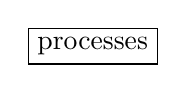
\begin{tikzpicture}
      \node [rectangle, text centered, draw=black]{processes};
    \end{tikzpicture},
    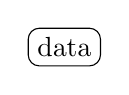
\begin{tikzpicture}
      \node [rectangle, rounded corners, text centered, draw=black]{data};
    \end{tikzpicture} and
    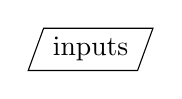
\begin{tikzpicture}
      \node [trapezium, trapezium left angle=70, trapezium right angle=110,
             text centered, draw=black]{inputs};
  \end{tikzpicture}}
  \label{figure:flow_chart}
\end{figure}

\section{Application}
\label{sec:application}

We have applied our methodology to evaluating QuickSpec, %TODO:cite
a library for conjecturing equations about functions in the Haskell programming
language. We use the Tons of Inductive Problems (TIP) theorem proving benchmark
to generate our corpus.

\subsection{QuickSpec}

We use QuickSpec version 0.9.6 to demonstrate our benchmarking methodology. This
is a library for the Haskell programming language, which is given a
\emph{signature} containing Haskell functions and (universally quantified) typed
variables, and outputs conjectured equations involving these terms.

The QuickSpec algorithm first enumerates all well-typed expressions, up to a
certain depth (3 by default), involving the given terms. Expressions of the same
type are assumed to be equivalent, and grouped into equivalence classes. A
testing process then tries to disprove this assumption by instantiating each
variable with a randomly chosen value (using the QuickCheck testing library),
evaluating the expressions and comparing the results. The equivalence classes
are split to separate any expressions which are observed to be different, and
the process repeats with new random values.

After 500 rounds of testing, any expressions still sharing the same equivalence
class are conjectured to be equal. Finally, a congruence closure algorithm is
applied to these equations, to find a minimal set.

In order to thoroughly benchmark QuickSpec, we need to automate some of the
decisions which are normally left up to the user:

\begin{itemize}
\item We must decide what variables to include. We add three for each type that
  appears as a function argument, except for types which have no QuickCheck data
  generator.
\item We must \emph{monomorphise} all types. For example, functions like
  \texttt{cons} are \emph{polymorphic}: they build lists of any element type.
  We need to pick a specific type in order to generate random values, so we
  resolve this, arbitrarily, by picking
  \emph{Integer}.~\footnote{We pick \texttt{Integer} for variables of kind
    \texttt{*}, and \texttt{[]} (Haskell's list type constructor) for those of
    kind \texttt{* -> *}. If these wouldn't satisfy some constraint, we pick a
    suitable type non-deterministically from the module scope, or skip these
    variables completely if none is found.}
\item Haskell functions only take one argument, as as in the $\lambda$-calculus,
  so functions of multiple arguments must be simulated by currying.
  Unfortunately QuickSpec cannot compare functions for equality, so we must give
  each function in our signature an explicit arity. Arities from zero to five
  are supported, so we avoid partial application by picking the highest that is
  type-correct.
\end{itemize}

To find out which functions to include in a signature, we use a plugin for the
GHC compiler which tells us all of the functions defined in a package. We
include all of those which type-check when passed to QuickSpec.

\subsection{TIP}

We use TIP version 0.2 which contains 343 problems, each stating a single
theorem and together defining a total of 618 datatypes and 1498 functions. Most
of these are duplicates, since each problem (re-)defines all of the datatypes
and functions it involves. We prefix the names of all definitions with the
filename it came from, and collect them into one big set.

Datatypes can have several ``constructors'' and ``destructors''. For example the
natural numbers can be defined as follows:

\begin{verbatim}
(declare-datatypes () ((Nat (Z) (S (p Nat)))))
\end{verbatim}

This defines the type \texttt{Nat}, along with the constructors \texttt{Z} (for
zero) and \texttt{S} (the successor function), and destructor \texttt{p} (the
predecessor function).

Since our GHC plugin only lists function definitions, we add separate function
definitions for each constructor and destructor (these are just
$\eta$-expansions).

TIP has ``native'' support for booleans and integers, allowing functions like
\texttt{+} to be used without an accompanying definition. Without a definition
these functions will not be included in the QuickSpec exploration, so we replace
all occurrences with custom definitions.

This gives us 3598 definitions in total, with 269 remaining after
$\alpha$-equivalent duplicates are removed.

TIP includes a tool to translate its definitions into Haskell code, including
suitable comparison functions and random data generators. We translated all 269
definitions into a single Haskell package, compiled it with GHC and extracted
the function definitions with our plugin. Each benchmark run imported this
entire package, but the signature given to QuickSpec only included functions
chosen for the current sample.

\subsection{Results}

\begin{figure}
  \includegraphics[width=8cm]{graphs/time}
  \includegraphics[width=8cm]{graphs/precRec}
  \caption{}
  \label{figure:quickspec_results}
\end{figure}

We applied our sampling methodology to the 269 TIP definitions for sample sizes
between 1 and 20, above which point QuickSpec becomes very slow. We chose 30
samples for each size, but the smaller sizes included repetitions due to the
requirement for samples to admit at least one theorem. The results are shown in
figure~\ref{figure:quickspec_results}.

Precision and recall were calculated by normalising each equation generated by
QuickSpec: all variables are identified numerically, in ascending order from
left to right; equations were also sorted such that the expression on the
left-hand-side is lexicographically smaller than that on the right.

Theorem statements from TIP were first updated to reference only the 269
distinct names we explored, and references to constructors and destructors were
updated to use the $\eta$-expanded versions instead. Equations were normalised
in the same way as above (non-equations were kept unchanged), and elements of
these two sets were deemed to match if they were syntactically identical.

We have applied our benchmarking methodology to the Tons of Inductive Problems
(TIP) problem set for automated theorem provers. TIP satisfies the desiderata of
section\ref{section:prep} since each problem has standalone type and function
definitions, making their separation trivial. The problem set includes known
examples from the software verification and inductive theorem proving
literature, including higher-order functions, common datatypes, etc., ensuring
that benchmark results are relevant to those fields. It also includes tools to
convert the problems into a variety of languages, including Haskell and
Isabelle.

TIP version 0.2 contains FIXME theorem statements, each of which is accompanied
by definitions of the types and functions it uses (other than those for integers
and booleans, which are ``built in''). There are FIXME function definitions, of
which most are duplicates. We remove $\alpha$-equivalent definitions in the
following way:

\begin{enumerate}
\item We prefix all type and function names with the filename in which we found
  the definition, so that e.g. the theorem statement from
  \texttt{tip2015/int\_add\_assoc.smt2} references the \texttt{plus} function from
  that file, rather than e.g. the \texttt{plus} function from
  \texttt{isaplanner/prop\_07.smt2}.
\item For each definition, all local variables (including function arguments,
  constructor parameters, pattern-matching variables and \texttt{let} bindings)
  are replaced by standard names \texttt{local-1}, \texttt{local-2}, etc. in a
  well-defined order.
\item An $O(n^2)$ comparison of each definition to every other definition is
  performed, to find any which are syntactically-identical modulo the names
  being defined (but \emph{not} the names being referenced, i.e. ). For those which are,
  we record which names are equivalent, replace all references to these names
  with whichever is smallest lexicographically, and remove
\end{enumerate}

Altogether TIP problem by QuickSpec and IsaCoSy theory
exploration systems. To assess the scalability of their algorithms, we sampled
theories of various sizes: from theories containing only a single definition, up
to theories containing 20 definitions.
 We call the Theory Exploration Benchmark (TEB).

To do this we can take a set of ATP tasks, for example proving the equation
\ref{eq:mapreduce} from the theory in figure \ref{figure:list_theory}, and we
split apart the definitions (to form a theory) from the theorem statements (to
form our ground truth).

We focus on the Tons of Inductive Problems (TIP) theorem proving
benchmark~\cite{claessen2015tip}, since it has several desirable properties:

All together, TIP provides 219 distinct function definitions and 343
  theorem statements, which is enough to fully exercise current ATE systems.
Benchmark problems include examples from the theorem proving literature
  as well as common program verification tasks, ensuring the resulting corpus is
  relevant to researchers and practitioners.
TIP's maintainers provide a set of tools, including translators from TIP's
  native format (based on SMT-Lib~\cite{BarFT-SMTLIB}) to Haskell and Isabelle
  (which are used by ATE systems).

To aid reproducibility, we use a cryptographic hash as our source of randomness:
the $n$th sample of size $s$ uses the SHA256 hash of $n$, $s$ and the definition
corpus; the latter prevents tailoring the corpus to influence the choices,
although ATE systems could .

To provide a more robust comparison of these two systems, we also applied a
paired difference test: measuring, for each sampled theory, the difference in
time, precision and recall between the two systems.

\section{Discussion}
\label{sec:discussion}

We are assuming that the ATE system acts in ``batch mode'' (accepting
definitions, producing conjectures, then halting), rather than running
continuously or interactively. This holds for all of the systems we have
analysed

% philosophical bits

% We're assuming there is general agreement on what is "good maths", when
% actually this isn't at all clear-cut

\section{Conclusion}
\label{sec:conclusion}

% future work, etc.

Our benchmark suite provides a unifying goal for the diverse approaches of
theory exploration, whilst avoiding some of the philosophical complications of
the field. Whilst the current implementation is quite limited, we welcome
additions from other researchers, to more closely align the benchmark with their
goals, and the strenghts and weaknesses of their systems.

``Solving'' this benchmark suite would not solve the problem of theory
exploration in general, so more ambitious goals must be set in the future; but
we have found that there is still a long way to go until that problem arises.

\begin{acknowledgements}
  We are grateful to Jianguo Zhang for help with our statistical analysis.

  EPSRC
\end{acknowledgements}

\bibliographystyle{plain}
\bibliography{./Bibtex}

\end{document}
